\documentclass{article}
\usepackage{tikzlings}
\usepackage{tikzlings-sheep}

% does not work
%\newcommand{\sheephookbelly}{%
%\fill[red!80!black]
%(0.55, 1.35) -- (0.65, 0.3) --
%(-0.65, 0.3) -- (-0.55, 1.35)
%-- (0.0, 0.9) -- cycle;
%}
%\sheep

\begin{document}
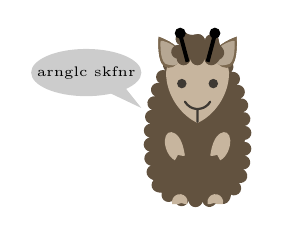
\begin{tikzpicture}

% \sheep[crown]

% \sheep[harlequin=blue, niuqelrah=red]

\sheep[alien=black,speech={\tiny{arnglc skfnr}},bubblecolour=gray!40!white]

% works
% \sheep[rotate=30,scale=0.5]
% \sheep[body=blue]
% \sheep[3D]
% \sheep[eye=red]

% does not work
% \sheep[blush]
% \sheep[back]
% \sheep[rotatearms=40]

\end{tikzpicture}



\begin{tikzpicture}
    \sheep[back]
\end{tikzpicture}

\end{document}